% ctexart、ctexrep、ctexbook和ctexbeamer, 对应 LaTeX 的article、report、book和beamer
\documentclass{article}
\usepackage[UTF8]{ctex}
\usepackage[a4paper,left=3cm,right=3cm,top=2.6cm,bottom=2.6cm]{geometry} % 设置页面尺寸
\usepackage{fancyhdr} % 设置页眉页边页脚
\usepackage{multicol} % 多栏排版
\usepackage{xeCJK} % 中文支持
\usepackage{ctex} % 中文支持
\usepackage{footmisc} % 控制脚注格式,包括编号、字体、分隔线等
\usepackage{titletoc} % 定制目录列表样式
\usepackage{fontspec} % XeTeX下的字体选择宏包
\usepackage{setspace} % 行距
\usepackage{graphicx} % 插图
\usepackage{pdfpages} % 引用pdf页面
\usepackage{booktabs} % 三线表
\usepackage{multirow} % 表格多行支持
\usepackage{caption} % figure和table等中的说明文字
\usepackage{tikz} % 绘图
\usepackage{etoolbox} % 给宏包打补丁
\usepackage{hyperref} % 超链接
\usepackage{xcolor} % 颜色支持
\usepackage{array} % 数学表格
\usepackage{amsmath} % 数学公式
\usepackage{amssymb} % 数学字体与符号
\usepackage{amsthm} % 数学定理格式
\usepackage{subfig} % 排版子图
\usepackage{float} % 浮动体格式控制
\usepackage{lmodern} % 一种字体支持
\usepackage{listings} % 插入代码
\usepackage{tcolorbox} % 好看的块环境
\usepackage{pifont} % 字体支持
\usepackage{perpage} %the perpage package
\usepackage{mathdesign} % some math fonts
\usepackage{ulem} %一些文字强调的宏包
\usepackage{fancyvrb} % some fancy verbatim 
\usepackage{enumitem} % 列表项目
\usepackage{txfonts} % 一些字体
\usepackage{makecell}
\usepackage{mathrsfs}
\usepackage{subfig}                 % 子图包,不要与{subfigure}混用,{subfig}较新
\usepackage{overpic}   
\usepackage{listing}   

%重置每页脚注序号
\MakePerPage{footnote} %the perpage package command
\renewcommand \thefootnote{\ding{\numexpr171+\value{footnote}}}
\pagestyle{headings} 
% 为tcolorbox导入三个程序包
\tcbuselibrary{skins, breakable, theorems} 

% 设置代码格式 - 关键字加粗, 其余为正常。非彩色
\lstset{
    aboveskip=5mm,
    belowskip=5mm,
    breaklines=true,
    breakatwhitespace=true,
    columns=flexible,
    extendedchars=false,
    showstringspaces=false,
    numbers=none,
    basicstyle={\small\ttfamily},
    captionpos=t,
    frame=tb,
    tabsize=4
}

\lstdefinestyle{cpp} {
  language=C++
}

\lstdefinestyle{c++} {
  language=C++
}

\lstdefinestyle{python} {
  language=python,
  morekeywords={as}
}

% 为目录添加 PDF 链接
\addtocontents{toc}{\protect\hypersetup{hidelinks}}

% 设置「目录」二字格式
\renewcommand{\contentsname}{
  \fontsize{16pt}{\baselineskip}
  \normalfont\heiti{目~~~~录}
  \vspace{-8pt}
}

% 定理、定义、证明
\newtheorem{theorem}{定理}[section]
\newtheorem{definition}{定义}[section]
\newtheorem{lemma}{引理}[section]
\newtheorem{corollary}{推论}[section]
\newtheorem{example}{例}
\newtheorem{proposition}{命题}[section]

\title{题目}
\author{作者}
\date{\today}

\begin{document}

% 显示标题作者时间
\maketitle
\newpage

% 调整目录行间距
\renewcommand{\baselinestretch}{1.35}
% 添加目录
\tableofcontents
\newpage

% 正文 22 磅的行距
\setlength{\parskip}{0em}
\renewcommand{\baselinestretch}{1.53}


\section{课题背景及意义}

\subsection{电磁干扰简介}
随着电子技术和信息化的发展,电磁波在各个领域广泛应用,但也造成了严重的电磁环境污染和电磁干扰问题。电磁波污染\textbf{不仅威胁着电子设备的正常运行和信息安全,也危害着人类的健康和生态平衡}。
因此,对其干扰的抑制和屏蔽的研究和应用具有重要的意义和价值。
\subsection{电磁波的危害}
电磁波对人体和环境都有不同程度的危害,主要表现在以下方面:
\begin{itemize}
\item 电磁波会对人体细胞组织产生生物效应,如局部热效应和非热效应,导致细胞功能紊乱、基因突变、免疫力下降等,增加患癌症、白血病、神经系统疾病等风险。
\item 电磁波会对人体生理心理产生影响,如头晕、失眠、记忆力减退、注意力分散、情绪不稳等,影响工作学习效率和生活质量。
\item 电磁波会对人体感觉器官产生刺激,如眼睛干涩、视力下降、听力损伤等,影响人体正常感知功能。
\item 电磁波会对环境生态产生干扰,如影响动物的迁徙和定向能力、影响植物的生长和开花能力、影响大气层和臭氧层的稳定性等,威胁自然平衡和资源可持续利用。
\end{itemize}
\subsection{电磁屏蔽及其意义}
\textbf{屏蔽设计是抑制电磁干扰的关键技术之一}。
通过屏蔽,可以把电磁能量限制在某一区域或使其不进入某个敏感区,有
效地切断干扰传播途径,实现设备和系统的电磁兼容性。

探索高效的电磁屏蔽材料科及合理的电磁屏蔽体的结构,防止电磁波辐射污
染以保护环境和人体健康,防止电磁波泄漏以保障信息安全,已经成为当前国
际上迫切需要解决的问题,各国已投入较多的人力物力,积极从事电磁波屏蔽
材料的研究和结构设计,多年来已陆续取得不少成果。
\subsection{电磁屏蔽具体应用}
        \begin{figure}[H]
            \centering
            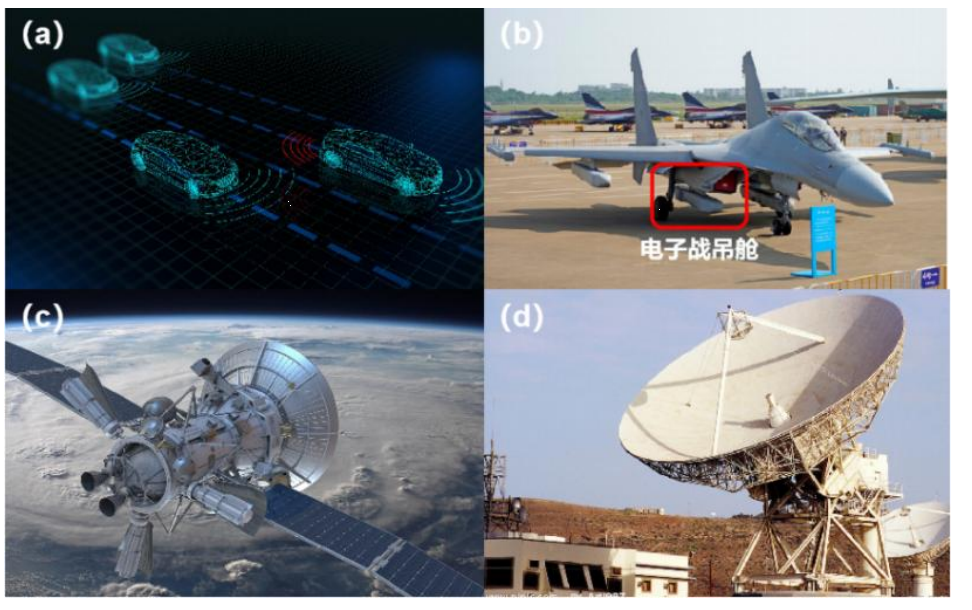
\includegraphics[width=8cm]{img/1.png}
            \caption{(a)自动驾驶雷达感知示意(b)J-16D 电子战机(c)高空通信卫星(d)军用 X 波
            段大功率雷达}
            \end{figure}
\subsubsection{国防安全领域}
以无人机、战斗机为代表的军事装备,最害怕的就是敌方的
电磁攻击和干扰,如果受到敌方强烈的电磁干扰,雷达便会失效,自身位置动向
也将被敌方先锁定,其根源因素也是机载雷达、电子元件无法对敌方的电磁干扰
进行有效的防护,而我国 J-16D 电子战机正是因为拥有超强的电子战吊舱,方才
具备对陆基、海基、空基通信系统(甚至是数据链系统)进行欺骗、干扰以及全
方位压制的能力,这也体现出在国防层面上,电磁屏蔽对于尖端装备的重要意义;

\subsubsection{航空航天领域}
空间站、高空雷达等设备由于处于外太空环境,多频率,多
方位的各类电磁波无时无刻不在对它们产生干扰,在复杂的电磁波环境下,航空
航天装备的电磁屏蔽材料更为重要,十分需要制作防护结构的电磁屏蔽材料其
屏蔽波段尽量广,屏蔽效能尽量高。
\subsubsection{民用领域}
汽车无人驾驶是目前关注最为火热的焦点,然而以特斯拉 FSD
为代表的无人驾驶技术发生了多起事故,这导致了人们极大的担忧。根据美国高
速公路安全管理局(NHTSA)发布的一份特斯拉自动驾驶事故调查报告显示,
其自动驾驶失灵的原因很大一部分是由于车载雷达无法屏蔽掉干扰波段的电磁
波,导致汽车信息中枢接受信号时发生紊乱甚至错误而造成的;
\subsection{电磁屏蔽仿真及其意义}
电磁屏蔽仿真是利用计算机软件模拟电磁场的分布和屏蔽材料的特性,以评估电子设备的电磁兼容性和屏蔽效能。

电磁屏蔽仿真的意义在于:
\begin{enumerate}[label=$\vardiamondsuit$,nosep]% nosep表示没有垂直间隔
    \item 可以节省实验成本和时间,避免复杂的实验条件和设备
    \item 可以探索不同的屏蔽方案和材料组合,优化屏蔽结构和性能
    \item 可以服务于社会生活、国民经济和国防工业,防止电磁波辐射污染和泄漏,保护环境和人体健康,保障信息安全
\end{enumerate}

电磁屏蔽仿真的原理是基于麦克斯韦方程组和有限元法,通过建立合理的仿真模型和边界条件,求解电磁场的分布和屏蔽材料的响应,计算屏蔽效能的指标。

电磁屏蔽仿真的过程一般包括以下步骤:
\begin{description}[leftmargin=4.7cm,style=nextline,nosep]% nosep没有垂直间隔
\item[选择合适的仿真软件和模块]如Ansoft HFSS1、Ansoft Maxwell3D4等。
\item[建立仿真模型]包括屏蔽体、信号源、接收器等。
\item[定义材料属性]如相对磁导率 μr​、相对介电常数 ϵr​、电导率 σ等。
\item[设置边界条件]如电壁、磁壁、吸收层等。
\item[进行网格划分和求解器选择]如有限元法、有限差分法等。
\item[后处理分析]如显示磁力线、磁通密度、屏蔽效能等。 
\end{description}

\section{问题的提出及其物理模型}
\subsection{蕴含的电磁问题}
为了便于分析计算,我们对电磁屏蔽问题做适当简化,可得以下问题。
\begin{quote}
{\qquad\parindent2\ccwd\kaishu\zihao{5}
将均匀介质球壳置于均匀外磁场$ H_{0} $中,介质的磁导率$ \mu$。
壳内外区域的磁导率为$ \mu_{0} $ 球壳的内、外半径分别为$ R_{1} $ 和 $ R_{2}$,
试求球壳内外空间的磁标势分布以及球壳内外的磁场强度
        \begin{figure}[H]
            \centering
            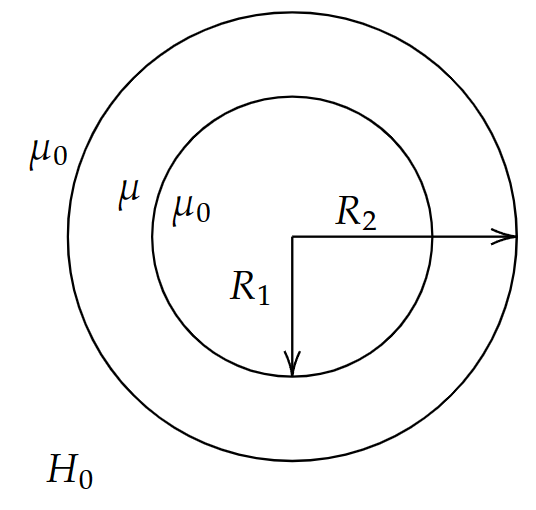
\includegraphics[width=4cm]{img/2.png}
            \caption{题图}
            \end{figure}
}
\end{quote}
\subsection{求解}
采用球坐标系,将空间分为三个区域,即$ r>R_{2},R_{1}<r<R_{1},r<R_{1}$
由于三个区域均无电流分布,均可使用磁标势法求解,$ r>R_{2} $ 区域的磁标势为$ \varphi_{m1},R_{1}<r<R_{2} $
区域的磁标势为$ \varphi_{m2},r<R_{1} $区域的磁标势为 $ \varphi_{m3} $。则三个区域满足的拉普拉斯方程为
\begin{align}
 \nabla^{2}\varphi _{m1}&=0(r>R_{2})\tag{2.1.a}\\  
 \nabla^{2}\varphi _{m2}&=0(R_{1}<r<R_{2})\tag{2.1.b}\\  
 \nabla^{2}\varphi _{m3}&=0(r<R_{1}) \tag{2.1.c}
\end{align}
列出所有的边界条件如下
\begin{align}
\varphi_{m1}|_{r \rightarrow \infty}&=-H_{0}r \cos \theta \tag{2.2.a}\\  
\varphi_{m3}|_{r \rightarrow 0} &=\text{有限值}\tag{2.2.b}\\ 
\varphi_{m1}|_{r=R_{2}}&= \varphi _{m2}|_{r=R_{2}} \tag{2.2.c}\\ 
\mu_{0}\frac{\partial \varphi _{m1}}{\partial r}|_{r=R_{2}}&= \mu \frac{\partial \varphi _{m2}}{\partial r}|_{r=R_{2}} \tag{2.2.d}\\ 
\varphi_{m2}|_{r=R_{1}}&= \varphi _{m3}|_{r=R_{2}} \tag{2.2.e}\\ 
\mu \frac{\partial \varphi _{m2}}{\partial r}|_{r=R_{1}}&= \mu _{0}\frac{\partial \varphi _{m3}}{\partial r}|_{r=R_{1}} \tag{2.2.f} 
\end{align}
由于此问题具有球对称性, 磁标势与方位角无关
\begin{equation}
    \varphi_{m1}=(r, \theta)\hspace{0.5cm}  \varphi _{m2}(r, \theta)\hspace{0.5cm}   \varphi _{m3}(r, \theta)\tag{2.3}
\end{equation}
所以就可以求出其通解为
\begin{align}
    \varphi_{m1}(r, \theta)&= \sum _{n=0}^{\infty}(A_{n}r^{n}+ \frac{B_{n}}{r^{n+1}})P_{n}\cos \theta(r>R_{2}) \tag{2.4.a}\\
 \varphi_{m2}(r, \theta)&= \sum _{n=0}^{\infty}(C_{n}r^{n}+ \frac{D_{n}}{r^{n+1}})P_{n}\cos \theta(R_{1}<r<R_{2}) \tag{2.4.b}\\
\varphi_{m3}(r, \theta)&= \sum _{n=0}^{\infty}(E_{n}r^{n}+ \frac{F_{n}}{r^{n+1}})P_{n}\cos \theta(r<R_{1})  \tag{2.4.c}
\end{align}
根据边界条件,通解可简化为
\begin{align}
    \varphi_{m1}&=-H_{0}r \cos \theta + \frac{B_{1}}{r^{2}}  (r>R_{2})  \tag{2.5.a}\\
    \varphi_{m2}&=C_{1}r \cos \theta + \frac{D_{1}}{r^{2}}(R_{1}<r<R_{2}) \tag{2.5.b}\\
    \varphi_{m3}&=E_{1}r \cos \theta(r<R_{1})\tag{2.5.c}
\end{align}


将 (2.5.a) 式和 (2.5.b) 式分别代人 (2.2.c) 式和 (2.2.d) 式可得两个方程, 再将 (2.5.b) 式和 (2.5.c) 
式分别代人 (2.2.e) 式和 (2.2.f) 式又可得两个方程, 由这四个方程可解得四个待定常数。 
\begin{align}
B_{1}  = \frac{(\mu _{r}-1)(1+2 \mu _{r})(R_{2}^{3}-R_{1}^{3})}{(1+2 \mu _{r})(2+ \mu _{r})-2(\mu _{r}-1)^{2}(R_{1}/R_{2})^{3}}  H_{0} \tag{2.6.a}\\ 
E_{1}= \frac{9 \mu _{r}}{(1+2 \mu _{r})(2+ \mu _{r})-2(\mu _{r}-1)^{2}(R_{1}/R_{2})^{3}}H_{0} \tag{2.6.b} 
\end{align}
所以,球内外的磁标势分别为
\begin{align}
  \varphi_{m1}=-H_{0}r \cos \theta + \frac{(\mu _{r}-1)(1+2 \mu _{r})(R_{2}^{3}-R_{1}^{3})}{(1+2 \mu _{r})(2+ \mu _{r})-2(\mu _{r}-1)^{2}(R_{1}/R_{2})^{3}}\frac{H_{0}}{r^{2}}(r>R_{2}) \tag{2.7.a}\\
  \varphi_{m3}= \frac{-9 \mu _{r}}{(1+2 \mu _{r})(2+ \mu _{r})-2(\mu _{r}-1)^{2}(R_{1}/R_{2})^{3}}H_{0}r \cos \theta \tag{2.7.b}
\end{align}

球壳内外的磁场根据磁场强度H与磁标势的关系
\begin{align}
  H&=- \nabla \varphi _{m} \tag{2.8}
\end{align}

球壳内磁场为
\begin{equation}
  \begin{array}{l}
    H_{3}=-\nabla \varphi_{m 3}=-\left(\frac{\alpha}{\alpha_{r}} e_{r}+\frac{1}{r} \frac{\alpha}{\alpha \theta}\right) \varphi_{m 3} \\
    =\frac{9 \mu_{r}}{\left(1+2 \mu_{r}\right)\left(2+\mu_{r}\right)-2\left(\mu_{r}-1\right)^{2}\left(R_{1} / R_{2}\right)^{3}} H_{0}\left(\frac{\alpha}{\alpha_{r}} e_{r}+\frac{1}{r} \frac{\alpha}{\alpha \theta} e_{\theta}\right) r \cos \theta \\
    =\frac{9 \mu_{r}}{\left(1+2 \mu_{r}\right)\left(2+\mu_{r}\right)-2\left(\mu_{r}-1\right)^{2}\left(R_{1} / R_{2}\right)^{3}} H_{0}\left(\cos \theta \boldsymbol{e}_{r}-\sin \theta \boldsymbol{e}_{\theta}\right) \\
    =\frac{9 \mu_{r}}{\left(1+2 \mu_{r}\right)\left(2+\mu_{r}\right)-2\left(\mu_{r}-1\right)^{2}\left(R_{1} / R_{2}\right)^{3}} \boldsymbol{H}_{0} \quad\left(r<R_{1}\right)
    \end{array} \tag{2.9}
\end{equation}

\begin{equation}
  \mu_{r} \rightarrow \infty \quad \boldsymbol{H}_{3}=\frac{9}{2 \mu_{r}\left[1-\left(R_{1} / R_{2}\right)^{3}\right]} \boldsymbol{H}_{0} \rightarrow 0 \quad\left(r<R_{1}\right)\tag{2.10}
\end{equation}
\subsection{绘图}
使用matlab对求解的结果进行绘图,结果如下
        \begin{figure}[H]
            \centering
            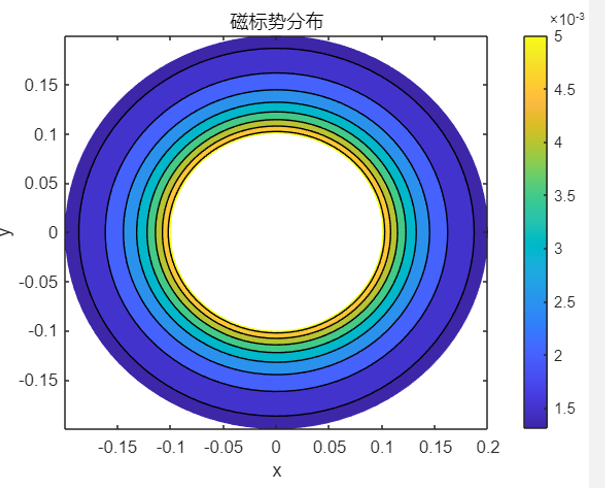
\includegraphics[width=8cm]{img/3.png}
            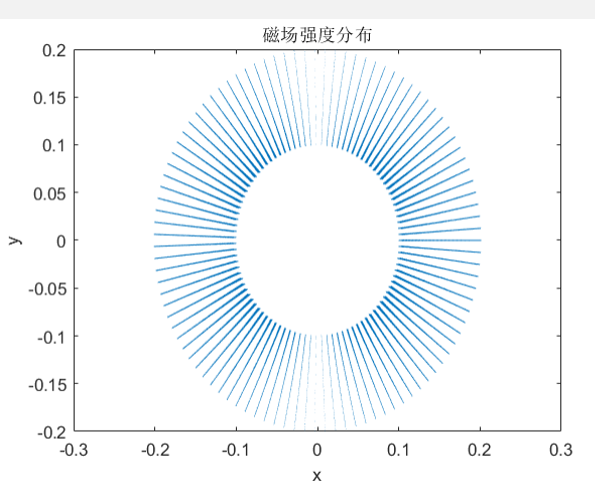
\includegraphics[width=8cm]{img/4.png}
\caption{球壳内磁标势示意图(matlab绘制)}
            \end{figure}
% \subsection{结果分析}
\subsection{静电场仿真(ANSYS Electromagnetic Suite)}
前面已经对静磁场屏蔽进行了仿真和计算,下面对静电场中球壳的屏蔽进行仿真。
        \begin{figure}[H]
            \centering
            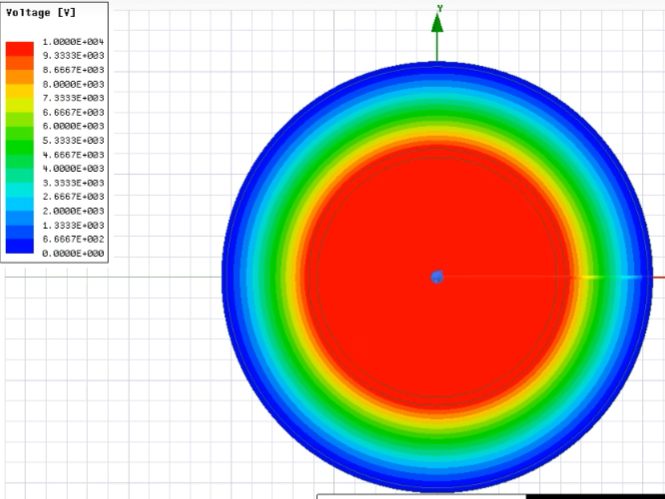
\includegraphics[width=12cm]{img/18.png}
          \caption{静电场仿真图}  
          \end{figure}
\section{结论}
\begin{equation}
  \mu_{r} \rightarrow \infty \quad \boldsymbol{H}_{3}=\frac{9}{2 \mu_{r}\left[1-\left(R_{1} / R_{2}\right)^{3}\right]} \boldsymbol{H}_{0} \rightarrow 0 \quad\left(r<R_{1}\right)\tag{3.1}
\end{equation}
根据上式,显然可知上试表明了磁场屏蔽原理,所选的$\mu_r$越大,球的壳层越厚,磁屏蔽效果就越好。
为了直观地展示我们地的结论,我们分别控制这两个变量画出图像,如下所示
        \begin{figure}[H]
            \centering
            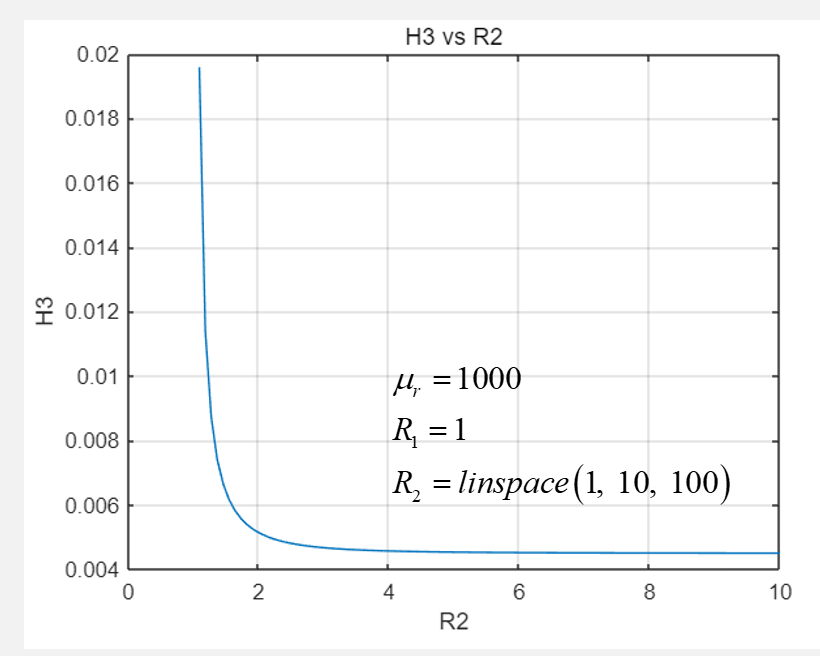
\includegraphics[width=12cm]{img/7.png}
            \caption[]{$R_2$变化}
            \end{figure}
            \begin{figure}[H]
              \centering
              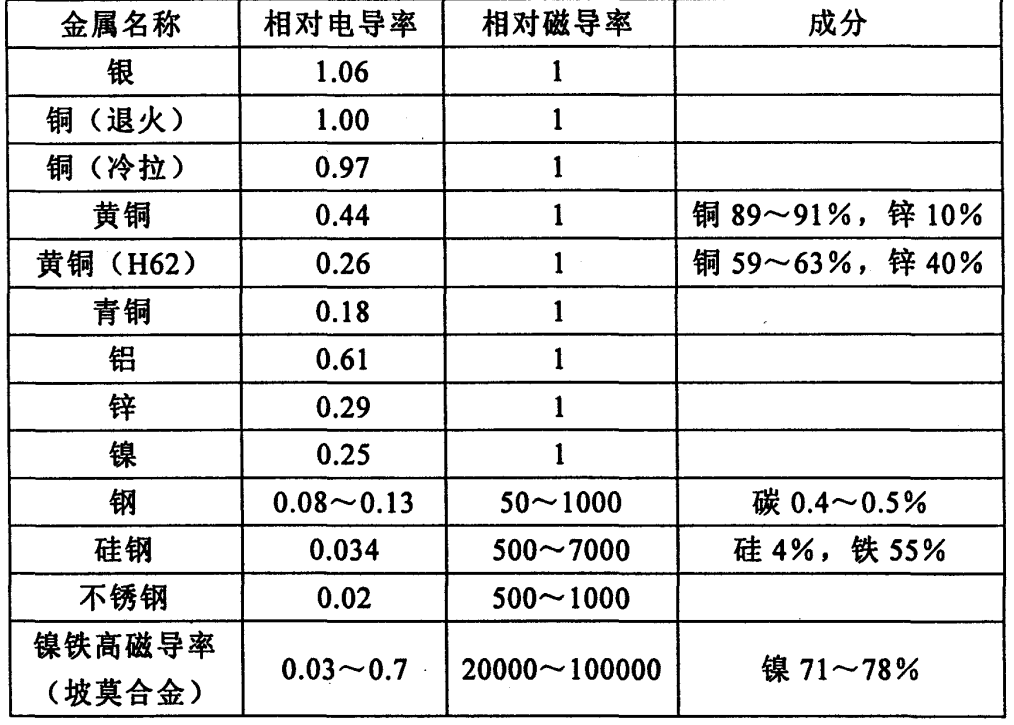
\includegraphics[width=12cm]{img/10.png}
              \caption[]{常用金属磁导率}
            \end{figure}
            \begin{figure}[H]
              \centering
              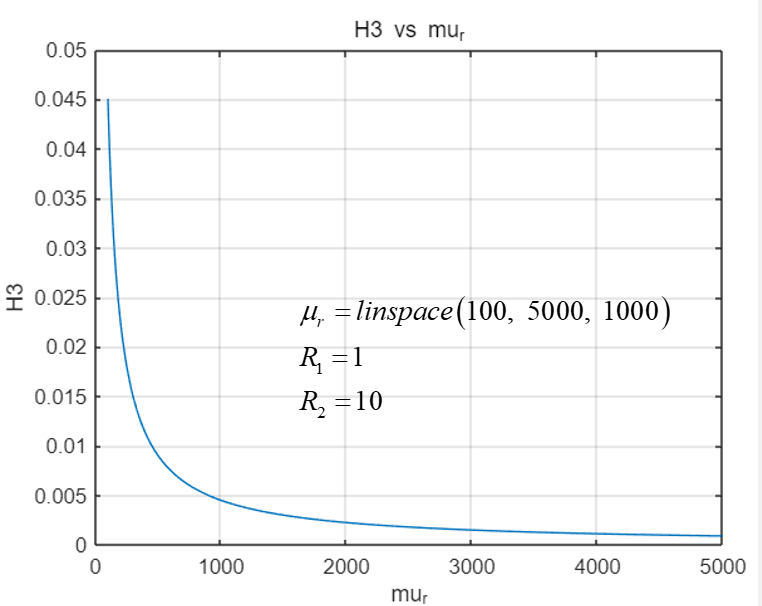
\includegraphics[width=12cm]{img/8.png}
              \caption[]{$\mu_r$变化}
              \end{figure}
\section{感悟和思考}
\subsection{感悟}
在本次报告的感悟思考部分,我想分享一下我个人在磁场屏蔽方面的学习与实践经验。

在研究磁场屏蔽的过程中,我采取了一些学习方法和工具,包括MATLAB仿真、
电动力学公式计算的复习,
以及Maxwell和ANSYS电磁场仿真软件的使用。这些工具和技术对我更深入地理解磁场屏蔽起到了积极的作用。

首先,MATLAB仿真是一个强大的工具,可以帮助我模拟和分析各种磁场屏蔽材料的性能。通过调整材料的参数和几何形状,我能够研究不同条件下的磁场屏蔽效果。这种仿真方法不仅提供了对材料性能的深入理解,还可以优化材料设计,并预测实际应用中的性能。

其次,复习电动力学公式的计算让我更好地理解了磁场屏蔽的基本原理。通过掌握电动力学知识,我能够推导与磁场屏蔽相关的公式,例如磁场分布和磁感应强度的计算公式。这些公式为我提供了评估和分析磁场屏蔽材料性能的依据。

在我的个人研究中,我也注意到磁场屏蔽在各个领域都有广泛的应用。不论是在航天领域还是手机等小型电子设备中,磁场屏蔽都扮演着重要的角色。例如,航天器需要在外界强磁场的干扰下正常运行,磁场屏蔽材料能够有效地减少外界磁场对设备的影响。同样地,在手机等电子设备中,磁场屏蔽可以降低电路之间的相互干扰,提高设备的性能和稳定性。

然而,我也意识到在磁场屏蔽材料领域,美国、日本等国家仍处于主导地位。为了推动本国产业的发展,我们应该抓住机会加速行业的发展,积极推进国产替代。通过加强研究与实践,我们可以提升本国磁场屏蔽材料的品质和性能,并在国内外市场上取得竞争优势。

总结而言,通过学习MATLAB仿真、复习电动力学公式计算以及使用Maxwell和ANSYS电磁场仿真软件,我在磁场屏蔽方面获得了宝贵的经验。我相信,通过持续的努力和创新,我们能够加速本国磁场屏蔽产业的发展,为社会提供更优质的磁场屏蔽解决方案。
\subsection{思考}
局限于这种结构为了增强其屏蔽性能,无非就做的特别大,或者改变其材料。所以当我们遇到瓶颈的时候,更多的还是去改变其材料,但是现有的材料无法满足,就需要去研究新型材料。

比如最近看到材化学院参加挑战杯的项目《国内首创超轻高强韧镁理基电磁屏蔽材料》就通过改变材料的方式来提高屏蔽性能,这种材料的研究还是很有意义的。
        \begin{figure}[H]
            \centering
            
\includegraphics[width=9cm]{img/11.png}
            \end{figure}

\section{附录}
\subsection{matlab代码(仿真图3)}
\begin{lstlisting}
  % 设置参数和几何结构
mu_0 = 4*pi*1e-7; % 真空中的磁导率
mu = 1.2e-6; % 介质的磁导率
R1 = 0.1; % 球壳的内半径(单位:米)
R2 = 0.2; % 球壳的外半径(单位:米)
H0 = 0.1; % 外磁场强度(单位:特斯拉)

% 设置模拟空间
num_points = 100; % 离散点数量
r = linspace(R1, R2, num_points); % 离散点的半径
theta = linspace(0, 2*pi, num_points); % 离散点的角度
[R, Theta] = meshgrid(r, theta); % 构建网格
;

% 初始化磁标势和磁场强度
A = zeros(num_points, num_points);
H = zeros(num_points, num_points, 2);

% 计算磁标势和磁场强度
for i = 1:num_points
for j = 1:num_points
r_val = R(i, j);
theta_val = Theta(i, j);
if r_val < R1 || r_val > R2

% 球壳内外区域
A(i, j) = -mu_0*H0*r_val*cos(theta_val); % 根据边界条件设置磁标势
H(i, j, 1) = 0; % 球壳内外区域的磁场强度为零
H(i, j, 2) = 0;
else
% 球壳内部
A(i, j) = -mu_0*H0*R1^2*cos(theta_val)/(2*r_val) + (mu_0*H0*R1^3)/(2*mu*r_val^2); % 根据边界条件设置磁标势
H(i, j, 1) = (mu_0*H0*R1^2*cos(theta_val))/(2*mu*r_val^2); % 计算球壳内的径向磁场强度
H(i, j, 2) = 0; % 球壳内的切向磁场强度为零
end
end
end


% 可以根据需要绘制磁标势和磁场强度的图像,例如:
% 绘制磁标势分布
figure;
contourf(R.*cos(Theta), R.*sin(Theta), A);
colorbar;
xlabel('x');
ylabel('y');
title('磁标势分布');

% 绘制磁场强度分布
figure;
quiver(R.*cos(Theta), R.*sin(Theta), H(:,:,1), H(:,:,2));
xlabel('x');
ylabel('y');
title('磁场强度分布')

\end{lstlisting}
\subsection{matlab代码(结果比较)}
\begin{lstlisting}

% 设置变量和参数
mu_r = linspace(100, 5000, 10000000);  % 磁导率相对值
R1 = 1;     % R1的值
R2 =10;   % R2的范围从1到10取100个点

% 计算H3
H3 = 9 ./ (2 * mu_r .* (1 - (R1 ./ R2).^3));

% 绘制曲线
plot(mu_r, H3)
xlabel('mu_r')
ylabel('H3')
title('H3 vs mu_r')
grid on

\end{lstlisting}
\subsection{ANSYS Electromagnetic Suite仿真过程}
        \begin{figure}[H]
            \centering
            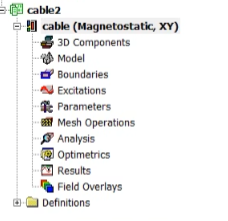
\includegraphics[width=12cm]{img/12.png}
          \caption[]{建立文件}  
          \end{figure}

          \begin{figure}[H]
            \centering
            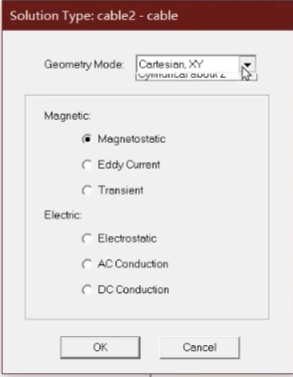
\includegraphics[width=12cm]{img/13.png}
          \caption[]{选择求解类型(选择静电场求解器)}  

          \end{figure}
          \begin{figure}[H]
            \centering
            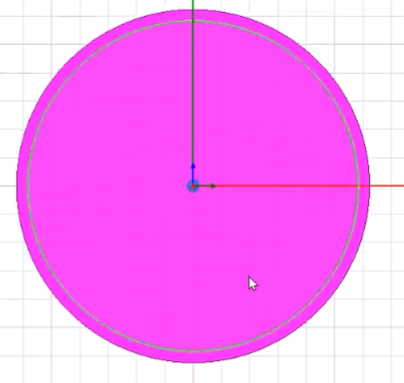
\includegraphics[width=8cm]{img/14.png}
            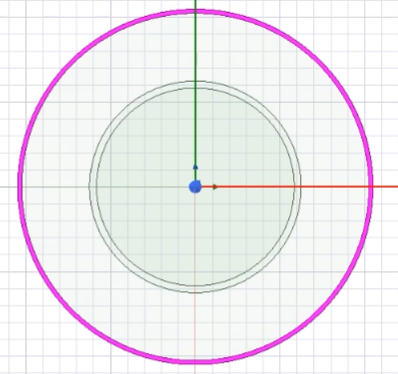
\includegraphics[width=8cm]{img/15.png}

          \caption[]{绘制球面}  
          
          \end{figure}
          \begin{figure}[H]
            \centering
            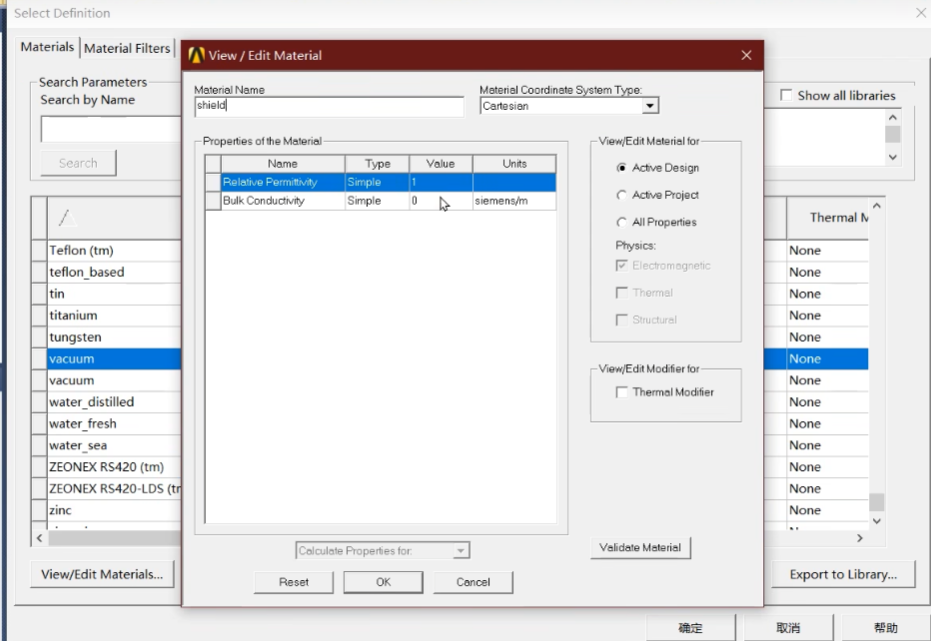
\includegraphics[width=8cm]{img/16.png}
          \caption[]{设置材料}  
          
          \end{figure}

          \begin{figure}[H]
            \centering
            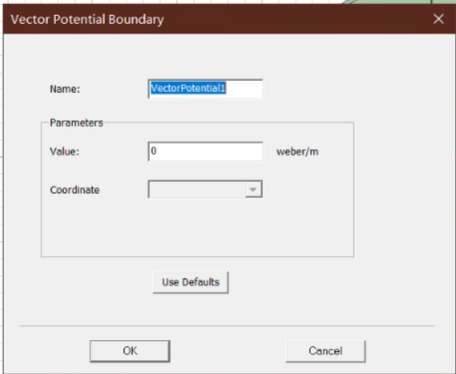
\includegraphics[width=8cm]{img/17.png}
          \caption[]{设置边界条件}  
          
          \end{figure}
          再检查模型正确性后,经过一系列后处理,得到仿真结果。
          \end{document}
